\def\difficulty{1}
\sujet{Histogram-based image segmentation}
\index{Segmentation!Histogram}
\index{Segmentation!Threshold}
\begin{note}This tutorial aims to implement some image segmentation methods based on histograms (thresholding and ``$k$-means'' clustering).\end{note}

\noindent The different processes will be applied on the following images:
{\makeatletter
	\renewcommand\fs@ruled{\def\@fs@cfont{\bfseries}\let\@fs@capt\floatc@ruled
		\def\@fs@pre{\hrule height.8pt depth0pt \kern2pt}%
		\def\@fs@post{\kern2pt\hrule\relax}%
		\def\@fs@mid{\vskip2pt}%
		\let\@fs@iftopcapt\iftrue}
	\makeatother
\begin{figure}[htbp]
\centering
\subfloat[Cells.]{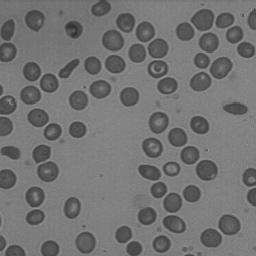
\includegraphics[height=4cm]{cells}}\hspace{1cm}
\subfloat[Muscle cells, author: Damien Freyssenet, University Jean Monnet, Saint-Etienne, France.]{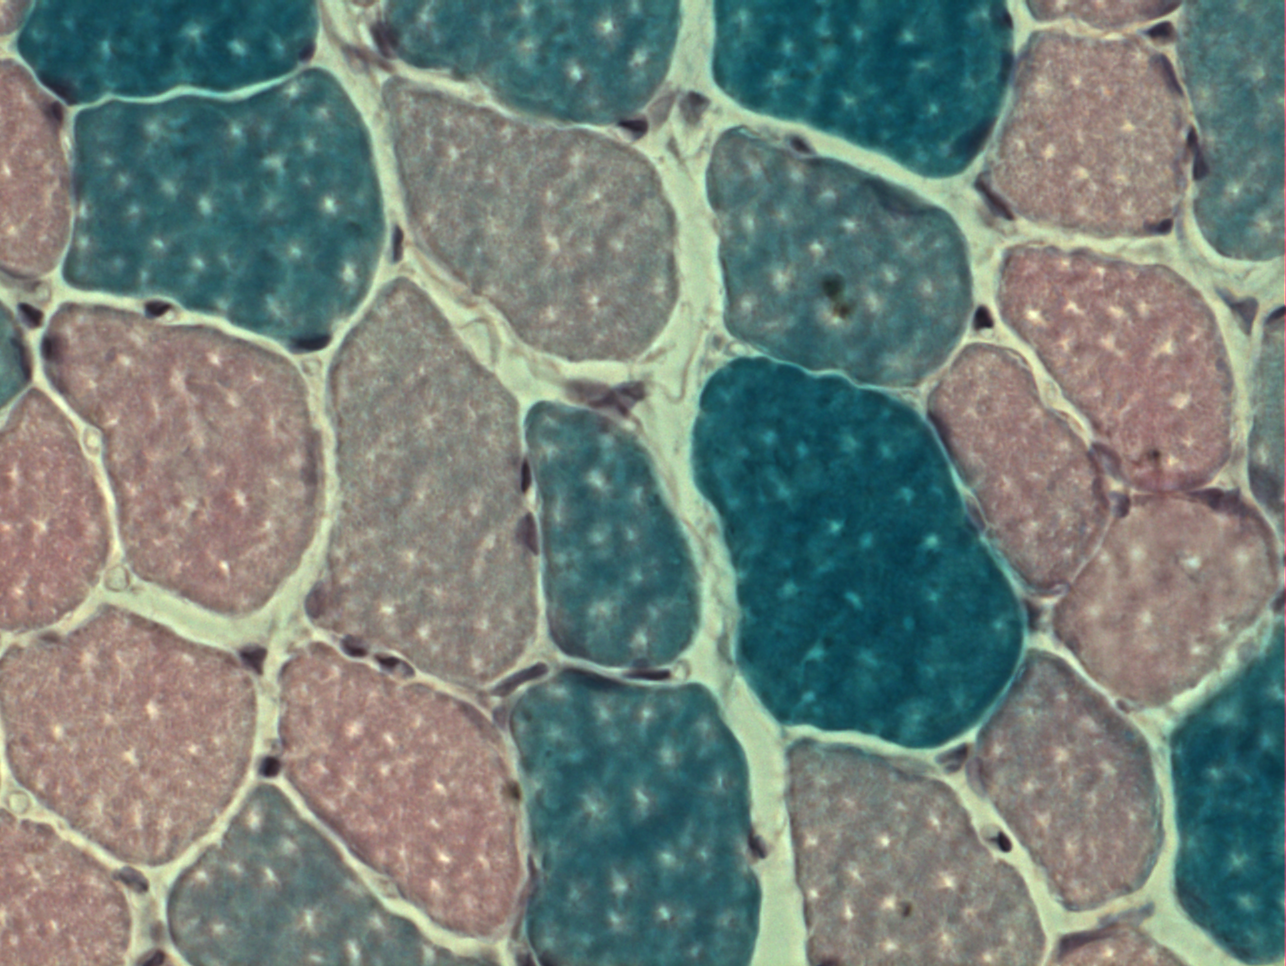
\includegraphics[height=4cm]{Tv16.png}}
\vspace*{-10pt}
\end{figure}}


\vspace*{-10pt}

\section{Manual thresholding}
The most simple segmentation method is thresholding.
\begin{qbox} 
\begin{itemize}
 \item Visualize the histogram of the grayscale image 'cells'.
 \item Make the segmentation with a threshold value determined from the image histogram.
\end{itemize}

\end{qbox}



\section{k-means clustering}
\index{Segmentation!K-means}
Let $X=\{x_i\}_{i\in [1;n], n\in \mathbb{N}}$ be a set of observations (the points) in $\R^d$. The $k$-means clustering consists in partitioning $X$ in $k\, (k<n)$ disjoint subsets $\tilde{S}$ such that:
\begin{equation}\tilde{S}=\displaystyle{\arg\,\min}_{S=\{S_i\}_{i\leq k}} \sum_{i=1}^{k} \sum_{x_j \in S_i} \left\|  x_j - \mu_i \right\|^2\end{equation}
where $\mu_i$ is the mean value of the elements in $S_i$. The $k$-means algorithm is iterative. From a set of $k$ initial elements $\{m_i^{(1)}\}_{i\in[1;k]}$ (randomly selected), the algorithm iterates the following $(t)$ steps:
\begin{itemize}
 \item Each element of $X$ is associated to an element $m_i$ according to a distance criterion (computation of a Voronoi partition):
\begin{equation}S_i^{(t)} = \left\{ \mathbf x_j : \big\| \mathbf x_j - \mathbf m^{(t)}_i \big\| \leq \big\| \mathbf x_j - \mathbf m^{(t)}_{i^*} \big\|, \forall i^*\in [1;k] \right\}\end{equation}

\item Computation of the new mean values for each class:\vspace*{-6pt}
\begin{equation} \mathbf m^{(t+1)}_i = \frac{1}{|S^{(t)}_i|} \sum_{\mathbf x_j \in S^{(t)}_i} \mathbf x_j\end{equation}
\vspace*{-\baselineskip}\vspace*{3pt}

\noindent where $|S^{(t)}_i|$ is the number of elements of $S^{(t)}_i$.
\end{itemize} 

\vspace*{-10pt}

\section{Grayscale image, $k=2$ in one dimension}

\vspace*{-6pt}

\index{Segmentation!Otsu thresholding}
The objective is to binarize image image 'cells', which is a grayscale image. The set $X$ is defined by $X=\{I(p)\}$, for $p$ being the pixels of the image $I$.
\begin{qbox}
\begin{itemize}
 \item 
Implement the algorithm proposed below (Alg. \ref{alg:histoseg:algo:threshold}).
\item Test this operator on the image 'cells'.
\item Test another method of automatic thresholding (defined by Otsu in \cite{Otsu1979}).
\item Compare the values of the thresholds (manual and automatic).
\end{itemize}
\end{qbox}

\begin{algorithm}[H]
\SetAlgoLined
\KwData{Original image $A$}
\KwData{Stop condition $\varepsilon$}
\KwResult{thresholded image}
 Initialize $T_0$, for example at $\frac{1}{2}(\max(A)+\min(A))$\;
	$done\leftarrow False$\;
	\While{ NOT $done$}{
	Segment the image $A$ with the threshold value $T$; \\
	it generates two classes $G_1$ (intensities $\geq T$) and $G_2$ (intensities $< T$)\;
	
	Compute the mean values, denoted $\mu_1, \mu_2$, of the two classes $G_1, G_2$, respectively\;
	
	Compute the new threshold value $T_i=\frac{1}{2}(\mu_1+\mu_2)$\;
	
	\If{$|T_i-T_{i-1}|<\varepsilon$}{$done\leftarrow True$}
	
	}
	
	Segment the image with the estimated threshold value.

\caption{K-means algorithm for automatic threshold computation of grayscale images.}\label{alg:histoseg:algo:threshold}
\end{algorithm}

\vspace*{-4pt}

\begin{mcomment}
\begin{mremark}
The Matlab function \texttt{graythresh} computes the automatic treshold by the method of Otsu. 
\end{mremark}
\end{mcomment}

\begin{pcomment}
\begin{premark}
For use with python, use the module \pinline{skimage.filter} and the function \pinline{threshold_otsu}.
\end{premark}
\end{pcomment}

\section{Simulation example, $k=3$ in two dimensions}

\vspace*{-6pt}%\enlargethispage{10pt}

The objective is to generate a set of 2-D random points (within $k=3$ distinct classes) and to apply the $k$-means clustering for separating the points and evaluating the method (the classes are known!).
\begin{qbox}
Write a function for generating a set of $n$ random points around a point with coordinates $(x,y)$.
 \end{qbox}

\vspace*{-4pt}

\begin{mcomment}
\begin{mremark}We will use the Matlab function \minline{randn}.\end{mremark}
\end{mcomment}
\begin{pcomment}
\begin{premark}We will use the python function \pinline{randn} from the module \pinline{numpy.random}.
\end{premark}
\end{pcomment}
 
\begin{qbox}
\begin{itemize}
\item Use this function to generate 3 set of points (in a unique matrix) around the points $(0,0)$, $(3,4)$ and $(-5,-3)$.

\begin{mcomment}
 \item  Use the Matlab function \minline{kmeans} for separating the points. The result is presented in Fig. \ref{fig:histoseg:kmeans}.
\end{mcomment}

\begin{pcomment}
 \item  Use the python function \pinline{sklearn.cluster.KMeans} for separating the points. The result is presented in Fig.\ref{fig:histoseg:kmeans}.
\end{pcomment}

\end{itemize}
 \end{qbox} 
\begin{mcomment}
\begin{mremark}Verify the utility of the option \minline{replicate}.  
\end{mremark}
\end{mcomment}
\begin{pcomment}
\begin{premark}
Verify the utility of the option \pinline{n_init=10}.
\end{premark}
\end{pcomment}

\vspace*{-8pt}

\begin{figure}[htbp]
\centering\caption{Resulting clustering of random points.}%
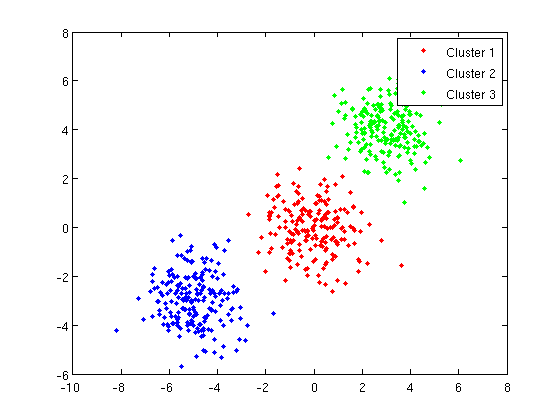
\includegraphics[width=9.5cm]{clusters.png}%
 \label{fig:histoseg:kmeans}%
\end{figure}

\vspace*{-8pt}

\section{Color image segmentation using K-means: $k=3$ in 3D}

The $k$-means clustering is now used for segmenting the color image representing the muscle cells 'Tv16.png'.

\begin{qbox}
Which points have to be separated? Transform the original image into a vector of size $N\times 3$ (where $N$ is the number of pixels) which represent the $3$ components R, G and B of each image pixel.
\end{qbox}

 \begin{mcomment}
\begin{mremark}The \matlabregistered{} function \minline{reshape} can perform the transformation.
 \end{mremark}
\end{mcomment}
\begin{pcomment}
\begin{premark}
The python function \pinline{numpy.reshape} does the same transformation.
\end{premark}
\end{pcomment}

\begin{qbox} 
 \begin{itemize}
 \item Visualize the 3-D map (histogram) of all these color intensities.
 \item Make the clustering of this 3-D map by using the K-means method. 
 \item Visualize the corresponding segmented image.
\end{itemize}
\end{qbox}
